Luego de haber consignado los requerimientos funcionales en la sección \ref{subsec:requerimientos_funcionales} y de haber formado, con ellos, la arquitectura tratada en el capítulo \ref{chap:arquitectura}, se retrató cada funcionalidad encontrada y que sería, a final de cuentas, soportada por el SNS en los casos de uso a continuación.

Los diagramas estarán dividos por cada módulo de gestión identificado basado cada uno en la especificación de requerimientos.

En \ref{app:cu_tablas}, el lector podrá encontrar la descripción de cada caso de uso en todos los módulos tenidos en cuenta en el SNS (los que se implementarán y los restantes).

\section{Módulo de gestión de administracion de deportes}


\begin{figure}[!htb]
  \begin{center}
    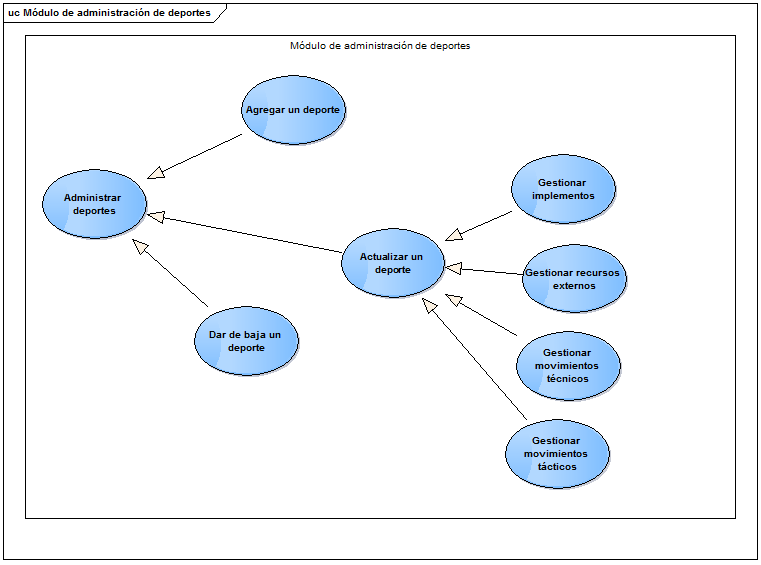
\includegraphics[width=11cm]{./imagenes/casos_uso/administracion_deportes.png}
    \caption{Módulo de gestión de administracion de deportes}
    \label{fig:cu_admin_dep}
    \textbf{Fuente:} Autores
  \end{center}
\end{figure}

Este módulo ofrece funcionalidades a los actores del sistema (especialmente el administrador) para administrar los deportes que éste juega, permitiendo al jugador dar información adicional de él en cada uno de los deportes que éste juega.

\section{Módulo de administración de eventos deportivos}

\begin{figure}[!htb]
  \begin{center}
    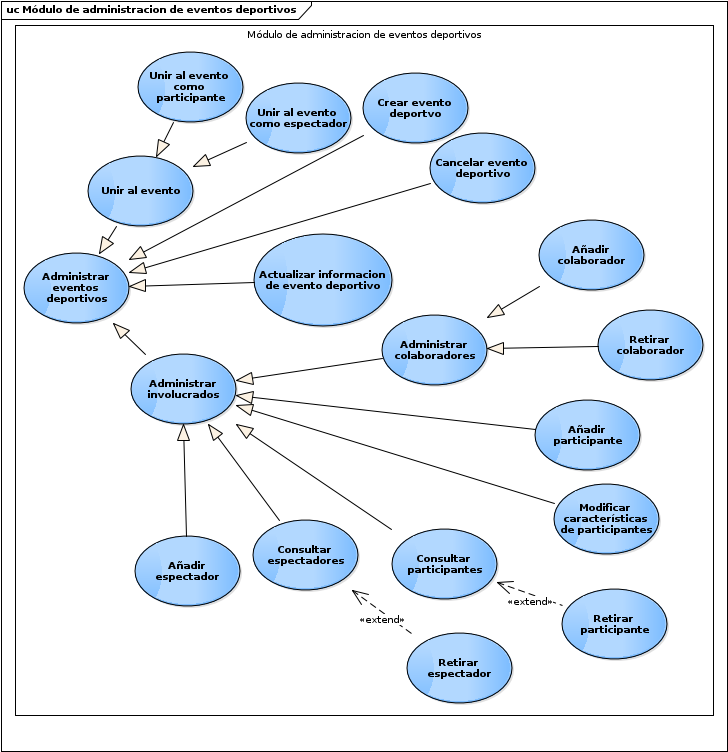
\includegraphics[width=11cm]{./imagenes/casos_uso/gestion_evento.png}
    \caption{Módulo de administración de eventos deportivos}
    \label{fig:cu_admin_eve}
    \textbf{Fuente:} Autores
  \end{center}
\end{figure}

En cuanto a éste módulo se refiere, los autores plasmaron las funcionalidades que se le ofrecen en el SNS a los organizadores de eventos deportivos, habiendo dos grandes módulos, a saber: Administración de involucrados y la gestión de la información del evento en si.

\section{Módulo de estadísticas}

\begin{figure}[!htb]
  \begin{center}
    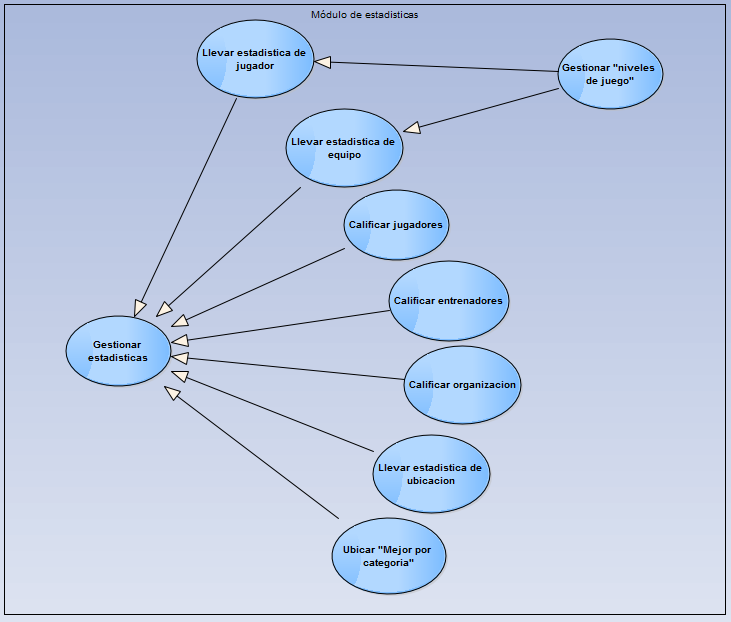
\includegraphics[width=11cm]{./imagenes/casos_uso/gestion_estadisticas.png}
    \caption{Módulo de estadísticas}
    \label{fig:cu_estad}
    \textbf{Fuente:} Autores
  \end{center}
\end{figure}

Las funcionalidades ofrecidas por éste módulo son proporcionadas por el SNS para dar soporte estadístico a cáda uno de los objetos de negocio especificados en el capítulo \ref{chap:arquitectura}, en lo que se refiere al proceso estadístico. Como adición, visto desde los requerimientos funcionales, se da una funcionalidad de llevar el mejor calificado en cáda uno de los objetos de negocio, con tal de que el usuario del SNS pueda ver aquellos objetos de negocio destacados cuando el lo requiera.

\clearpage

\section{Módulo de gestión de self-expression}

\begin{figure}[!htb]
  \begin{center}
    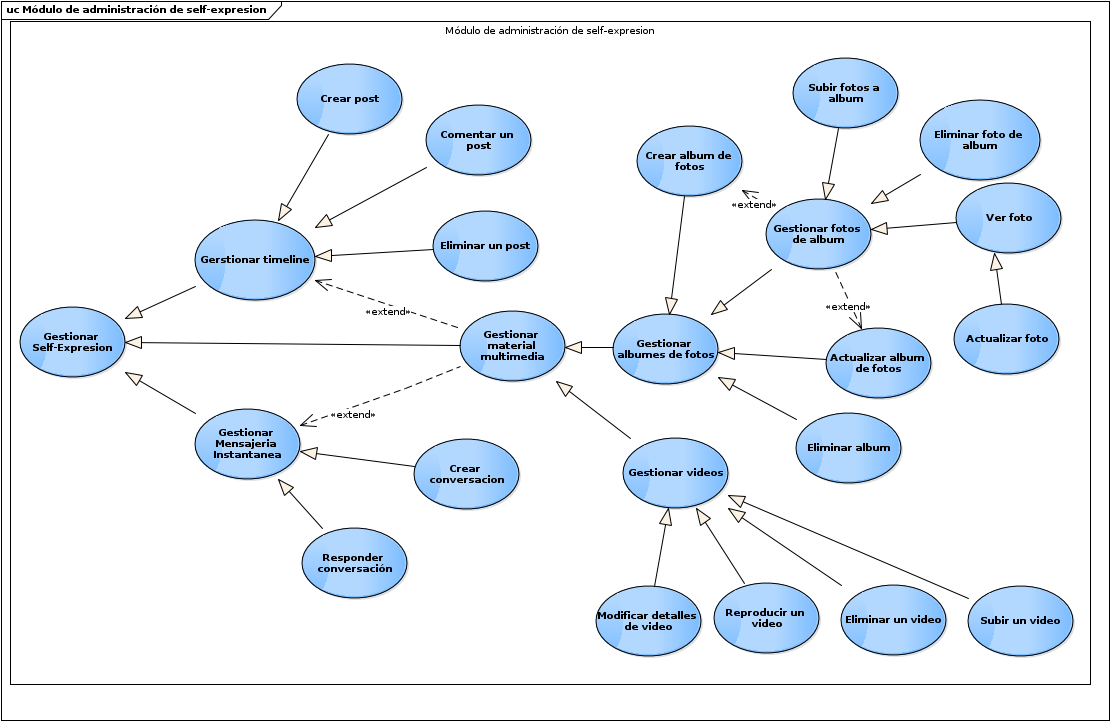
\includegraphics[width=11cm]{./imagenes/casos_uso/gestion_self_sharing.png}
    \caption{Módulo de gestión de self-expression}
    \label{fig:cu_self_shar}
    \textbf{Fuente:} Autores
  \end{center}
\end{figure}

Este módulo ofrece funcionalidades propias de redes social similares a Facebook. Por medio de éste el usuario podrá manejar la comunicación de él con sus amigos a traves de un timeline, del servicio de mensajería instantánea y de la posibilidad de compartir elementos multimedia como lo son videos y fotos, así como también mostrar y actualizar su información personal.

\section{Módulo de gestión del conocimiento}

\begin{figure}[!htb]
  \begin{center}
    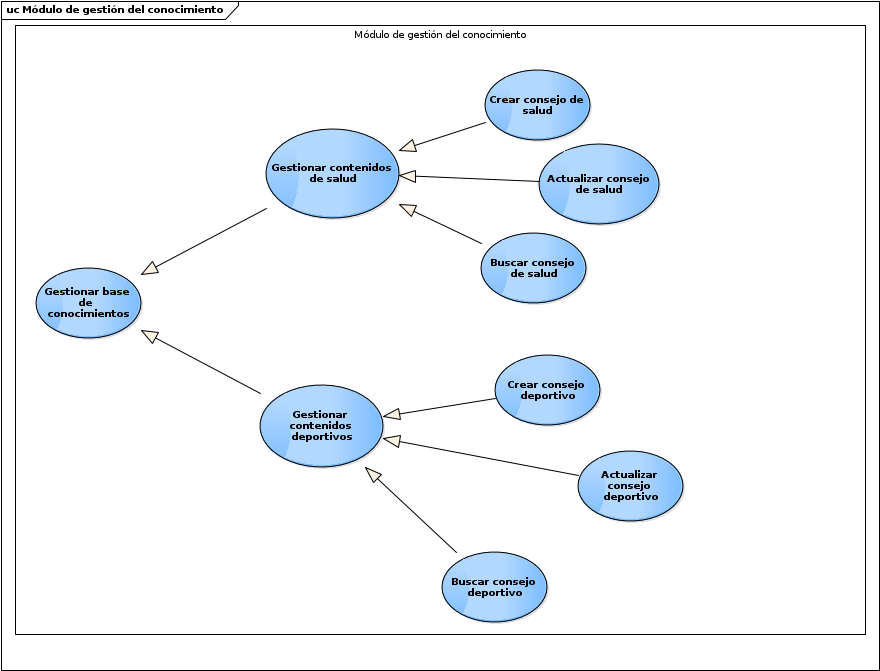
\includegraphics[width=11cm]{./imagenes/casos_uso/gestion_conocimiento.png}
    \caption{Módulo de gestión de self-expression}
    \label{fig:cu_self_shar}
    \textbf{Fuente:} Autores
  \end{center}
\end{figure}

Este modulo ofrece al usuario la funcionalidad de buscar o publicar información relacionada a los deportes. En el alcance actual se tiene contemplados contenidos deportivos (relacionados a la práctica de un deporte) y de salud (relacionados a consejos y cuidados orientados a los deportistas).

\section{Módulo de gestión de usuarios}

\begin{figure}[!htb]
  \begin{center}
    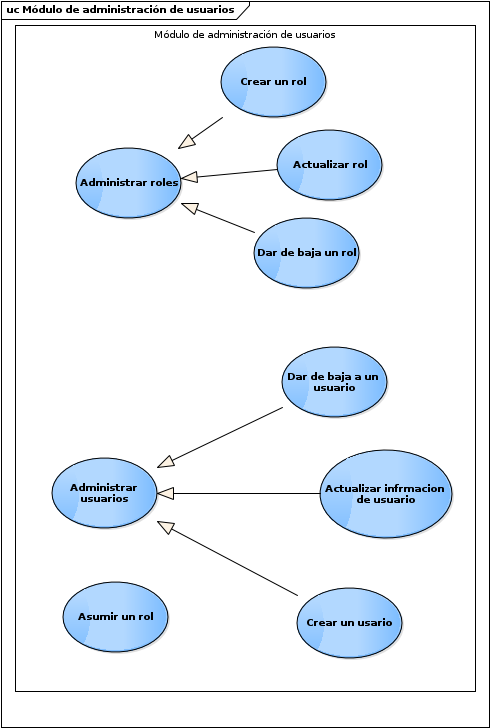
\includegraphics[width=11cm]{./imagenes/casos_uso/gestion_usuarios.png}
    \caption{Módulo de gestión de self-expression}
    \label{fig:cu_self_shar}
    \textbf{Fuente:} Autores
  \end{center}
\end{figure}

Este modulo ofrece a los usuarios la funcionalidad de administrar y gestionar su información como usuario de la aplicación (datos personales, datos de contacto)
